\documentclass[assignment03_Solutions]{subfiles}

\IfSubStr{\jobname}{\detokenize{Solutions}}{\toggletrue{solutions}}{\togglefalse{solutions}}

\fancypagestyle{firstpage}

{\rhead{Assignment 3 \linebreak \textit{Version: \today}}}

\title{Assignment 3: Probabilistic Definitions of Fairness and Text Classification}
\author{Machine Learning}
\date{Fall 2019}
\invalidatemargin

\begin{document}

\maketitle
\thispagestyle{firstpage}


\begin{learningobjectives}
\bi
\item Learn about the connection between probabilistic criteria for algorithmic fairness and Bayesian Networks.
\item Solidify your understanding of the Na\"ive Bayes algorithm by applying it to movie review sentiment classification.
\ei
\end{learningobjectives}

\section{Bayesian Networks and Algorithmic Fairness}


In assignment 1 of this module we discussed how Bayesian methods can be used to reason about algorithmic fairness.  We've just had some lengthy discussions about fairness within the context of the COMPAS algorithm.  We touched upon some of the limitations of statistically based notions of fairness.  Nevertheless, these criteria do have a potential role to play, and you should know what the most common definitions of fairness are and what assumptions they make.

As context for the reading and to help us have common notation, suppose we have the following random variables.

\bi
\item $R$ represents the prediction generated by our algorithm.
\item $A$ represents a sensitive attribute
\item $Y$ represents the thing we're trying to predict (we want $R = Y$ if we are accurate)
\ei

\todo replace maybe with Micah's stuff
\begin{externalresources}[(40 minutes)]
Read \href{https://fairmlbook.org/classification.html}{Fairness and Machine Learning Chapter 2}.  Start at the section \emph{Formal non-discrimination criteria} and read up to (but not including) the section \emph{Calibration and sufficiency}.
\begin{notice}
\bi
\item Don't get too hung up on the \href{https://en.wikipedia.org/wiki/Receiver_operating_characteristic}{ROC curves}.  We can discuss this on NB, but it is not required to understand what is going on here.  If you decide to check it out, you'll see an example of an ROC curve in the notebook linked below (it is optional).
\item The notation they use in this reading for conditional independence is $\bot$ (instead of our notation, $\condindep$).
\ei
\end{notice}
\end{externalresources}


\begin{exercise}[(10 minutes)]
Thinking back to the COMPAS example, which definition of fairness given in the reading was ProPublica using?  Which definition of fairness was Northpointe using?

\begin{boxedsolution}
\bi
\item Northpointe is using sufficiency $Y \condindep A~|~R$.  You'll notice that in the reading they say that sufficiency is the same thing as matching positive and negative predictive value for all values of the protected attribute.
\item Propublica is using separation $R \condindep A~|~Y$.  This fairness principle requires the false positive and true positive rates to be the same across for all values of the protected attribute.
\ei
\end{boxedsolution}
\end{exercise}

%If you're interested in examining the Broward County COMPAS data yourself, we have put together \href{https://colab.research.google.com/github/mlfa19/assignments/blob/master/Module\%202/03/Exploring_COMPAS_Data.ipynb}{a notebook that reproduces the calculations that are at the heart of the two competing notions of fairness}.  The notebook is written in with some notebook exercises, but these are totally optional.  We expect that the default will be that folks will just take a look if they want to (or skip this if they don't). If you want to spend some extra time and solidify your understanding of true positive rate, false positive rate, positive predictive value, etc., then it might be worth doing it as a set of exercises.


\section{Generative versus Discriminative Models}
In this assignment and the previous one we've built up a lot of machinery that allows us to work with probabilities.  Next we're going to take this machinery and turn back towards machine learning.  Specifically, we'll be looking at the classification problem and using probability theory to see it in a whole new light (who's excited?!?).


\subsection{Discriminative Models: a Look Back at Logistic Regression (10 minute read)}

Let's think back to the logistic regression model for binary classification that we learned about in module 1.  Given an input point $\mathbf{x_i}$, the logistic regression algorithm applied a weight vector $\mathbf{w}$ to compute the probability that the corresponding output $y_i$ was 1 via the formula $\sigma(\mathbf{w}^\top \mathbf{x_i}) = \frac{1}{1+e^{-\mathbf{w}^\top \mathbf{x_i}}}$ (recall that $\sigma$ is known as the sigmoid function and serves to squash its input into a number between 0 and 1, which can serve as a valid probability).  While we didn't quite have the vocabulary for it then, what we were really doing was computing a conditional probability.  We can think of $Y_i$ as a random variable that represents the output corresponding to the input $\mathbf{x_i}$ (in the case of binary classification $Y_i$ is either 0 or 1).  We can also think of the input as a random variable $X_i$ (thinking of the input as a random variable will be helpful later in this section).  Framed in this way the logistic regression algorithm computes the following conditional probability:
\begin{align}
p(Y_i = 1 | X_i = \mathbf{x_i}) &= \sigma(\mathbf{w}^\top \mathbf{x_i}) \enspace .
\end{align}

We defined a loss function to specify which weights were better or worse given a training set $(\mathbf{x_1}, y_1), (\mathbf{x_2}, y_2), \ldots, (\mathbf{x_n}, y_n)$.  The details of how we did this are not important to the point we are trying to make now, so it'll suffice to say that learning in a logistic regression model meant tuning the conditional distribution of the outputs (the $Y_i$'s) given the inputs ($\mathbf{x_i}$'s) to fit the training data the best.  This type of model is what is known as a \emph{discriminative model} (the \href{https://en.wikipedia.org/wiki/Discriminative_model}{Wikipedia article on discriminative models} has more details if you are interested).

\vspace{1em}

\begin{understandingcheck}
Intuitively, why does being able to accurately estimate $p(Y = 1 | X = \mathbf{x})$ allow you to classify unseen test data?

\begin{boxedsolution}
In a classification problem we are interested in predicting the output for a given input, $\mathbf{x}$.  If we can accurately calculate $p(Y=1|X = \mathbf{x})$, then we can simply threshold this value at $0.5$ (or whatever makes sense given our application) and predict $Y = 1$ if this condition is met and $Y = 0$ otherwise.
\end{boxedsolution}
\end{understandingcheck}

\subsection{Generative Models (10 minute read)}
The approach outlined above is great, but it's not the only way to approach binary classification (and supervised learning in general).  Since we are interested in predicting $Y_i$ given some inputs $\mathbf{x_i}$, it of course makes sense, for example for a binary classification problem, to want to determine $p(Y_i = 1 | \mathbf{x_i})$.  However, Instead of modeling that distribution directly, we can use Bayes' rule.

\begin{align}
p(Y_i  = 1 | X_i = \mathbf{x_i}) &= \frac{p(X_i = \mathbf{x_i} | Y_i = 1) p(Y_i = 1)}{p(X_i = \mathbf{x_i})} \label{eq:pgm} \\
&= \frac{p(X_i = \mathbf{x_i} | Y_i = 1) p(Y_i = 1)}{p(X_i =  \mathbf{x_i} | Y_i = 1) p(Y_i = 1) + p(X_i = \mathbf{x_i} | Y_i = 0) p(Y_i = 0)} \nonumber
\end{align}

These equations tell us is that if we have a model of the probability of the output being 1 \emph{a priori}, $p(Y_i = 1)$, and a model of the inputs $\mathbf{x_i}$ given the output $y_i$, $p(X_i = \mathbf{x_i} | Y_i = y_i)$, then we can compute $p(Y_i = 1 | X_i = \mathbf{x}_i)$.  This amounts to adopting the perspective that the hidden output $Y_i$ causes the input $X_i$.  We call this sort of model a \href{https://en.wikipedia.org/wiki/Generative_model}{probabilistic generative model} (PGM).  The BN corresponding to this model is given below.

\begin{center}
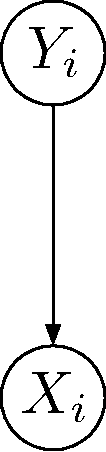
\includegraphics[width=0.05\linewidth]{figures/pgm}
\end{center}


The natural question is \emph{why?} Here are some potential advantages of using probabilistic generative models.
\bi
\item Suppose you found out that $p(Y_i)$ changed for some reason (any thoughts on when this might happen?  Post here on NB).  Incorporating this change into a probabilistic graphical model would be very straightforward (just modify $p(Y_i =1)$ in Equation~\ref{eq:pgm}).
\item Suppose you found out that $p(X_i  = \mathbf{x_i} | Y_i = y_i)$ changed for some reason.  For example, if one of the elements of $X_i$ represents a result obtained by running some sort of medical test, the sensitivity of that medical test might change (any other examples on when this might happen? Post here on NB.).
\item Suppose that instead of classifying data (i.e., predicting $Y_i$), you instead wanted to generate samples $\mathbf{x_i}$ conditioned on a particular value of $Y_i$ (e.g., you might want to \href{https://www.youtube.com/watch?v=LzE1fF0_3q0}{synthesize samples of hand written digits} based on training a probabilistic graphical model).  This can be done naturally with a PGM.  More modern versions of this idea are generative adversarial networks (GANs), which are behind such work as this \href{https://thispersondoesnotexist.com/}{person does not exist} and \href{https://openai.com/blog/better-language-models/}{better language models and their implications} (the second link is the work of a former Oliner!).
\ei

\begin{understandingcheck}
What are the probabilities needed to classify input data in a discriminative model?  What are the probabilities needed to classify input data in a generative model?  How does Bayes' rule connect these two models?

\begin{boxedsolution}
For a discriminative model you need $p(Y=1 | X = \mathbf{X})$.  For a generative model you need $p(Y=1)$ and $p(X = \mathbf{x} | Y=1)$.  Bayes' rule provides the linkage between these two models since one can be transformed into the other simply by applying Bayes' rule.
\end{boxedsolution}
\end{understandingcheck}


\section{Meet the Na\"ive Bayes Algorithm}
Now that we've learned the basic concept of a probabilistic graphical model, let's make things concrete and learn about a specific PGM.  For our first PGM, we're going to learn about the Na\"ive Bayes algorithm (we'll be doing some work with Na\"ive Bayes in the next assignment as well, so you'll have some time to get accustomed to it).  The reason it is called Na\"ive Bayes is that it assumes that all of the observed data ($X_1, X_2, \ldots, X_n$) are conditionally independent given $\mathcal{Y}$.  The BN for the Na\"ive Bayes algorithm is shown below.
\begin{center}
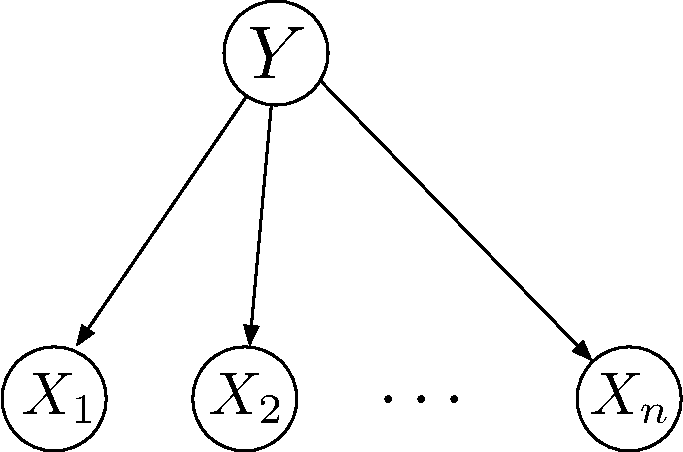
\includegraphics[width=0.3\linewidth]{figures/naivebayesgm}
\end{center}

As a motivating example, let's look back at the Titanic dataset from the last module.  A potential BN for the Titanic dataset is shown below.

\begin{center}
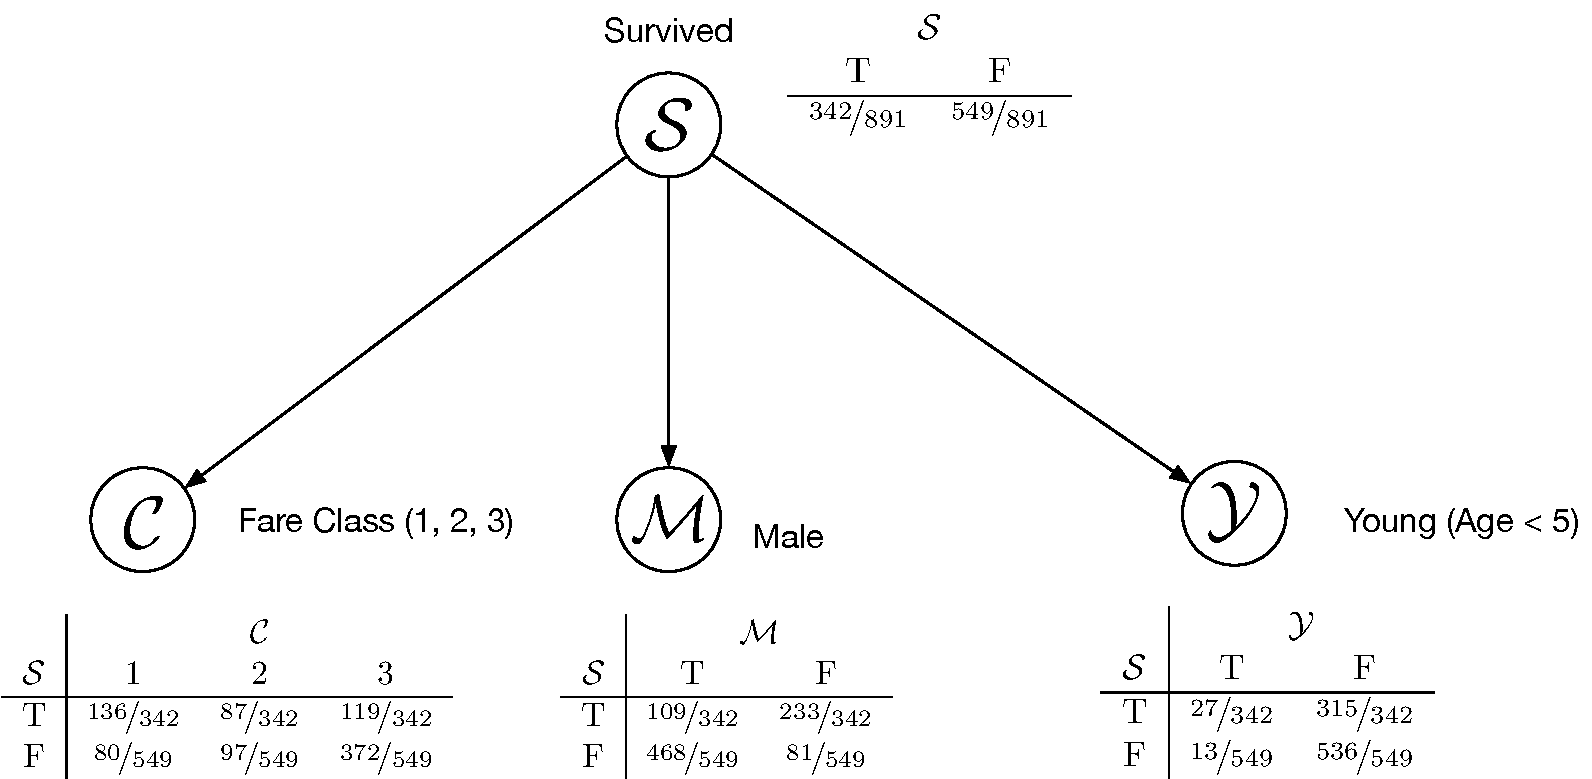
\includegraphics[width=0.8\linewidth]{figures/titanicbn}
\end{center}

The probabilities in this BN were computed by looking at the training set and counting the appropriate passengers that fell into each category.  For instance, to compute $p(\mathcal{Y}|\mathcal{S})$ since $p(\mathcal{Y}|\mathcal{S}) = \frac{p(\mathcal{Y}, \mathcal{S})}{p(\mathcal{S})}$, we can approximate this probability by counting the number of passengers under 5 who survived and dividing by the total number who survived (note that there are some subtle and important modifications to this method of fitting these probabilities that we'll discuss in the next assignment).  This process was repeated for each conditional probability.  Since we assume that all of the features are conditionally independent given the output ($\mathcal{S}$ in this case), this process is done independently for each feature.

\subsection{Inference}
While the Na\"ive Bayes Algorithm might sound fancy, once we have the BN, all we need to do to run the algorithm is to use Bayes' rule.  We'll let you work through this on your own via an exercise.

\begin{exercise}[(45 minutes)]

\bes
\item Using the BN shown above, what is the probability that a young, male in first class would survive the Titanic disaster?  Hint: write this as a conditional probability and then use Bayes' rule.  Hint 2: leverage the fact that $\mathcal{C}, \mathcal{Y}, \mathcal{M}$ are all conditionally independent of each other given $\mathcal{S}$.

You have just derived the Na\"ive Bayes inference rule!

\begin{boxedsolution}
\begin{align}
p(\mathcal{S}|\mathcal{Y}, \mathcal{C}=1, \mathcal{M}) &= \frac{p(\mathcal{Y}, \mathcal{C}=1, \mathcal{M}|\mathcal{S})p(\mathcal{S})}{p(\mathcal{Y}, \mathcal{C}=1, \mathcal{M})} \nonumber \\
&= \frac{p(\mathcal{Y}, \mathcal{C}=1, \mathcal{M}|\mathcal{S})p(\mathcal{S})}{p(\mathcal{Y}, \mathcal{C}=1, \mathcal{M}| \mathcal{S})p(\mathcal{S}) + p(\mathcal{Y}, \mathcal{C}=1, \mathcal{M}|\neg \mathcal{S})p(\neg \mathcal{S})} \nonumber \\
&=  \frac{p(\mathcal{Y}|\mathcal{S}) p( \mathcal{C}=1 | \mathcal{S}) p(\mathcal{M}|\mathcal{S})p(\mathcal{S})}{p(\mathcal{Y}|\mathcal{S}) p( \mathcal{C}=1 | \mathcal{S}) p(\mathcal{M}|\mathcal{S})p(\mathcal{S}) + p(\mathcal{Y}|\neg \mathcal{S}) p( \mathcal{C}=1 | \neg \mathcal{S}) p(\mathcal{M}|\neg \mathcal{S})p(\neg \mathcal{S})} \nonumber \\
&= \frac{\left ( \frac{27}{342} \times \frac{136}{342} \times \frac{109}{342}\times \frac{342}{891}\right)}{\left ( \frac{27}{342} \times \frac{136}{342} \times \frac{109}{342}\times \frac{342}{891} \right ) + \left ( \frac{13}{549} \times \frac{80}{549} \times \frac{468}{549}\times \frac{549}{891} \right )} \nonumber \\
&= 0.6794 \nonumber
\end{align}

\end{boxedsolution}

\item Na\"ive Bayes is often more conveniently expressed using odds ratios.  Instead of computing $p(\mathcal{S}|\mathcal{Y}, \mathcal{C}=1, \mathcal{M})$ let's compute the following.
\begin{align}
\frac{p(\mathcal{S}|\mathcal{Y}, \mathcal{C}=1, \mathcal{M})}{p(\neg \mathcal{S}|\mathcal{Y}, \mathcal{C}=1, \mathcal{M})} &= \frac{\frac{p(\mathcal{Y}, \mathcal{C}=1, \mathcal{M} | \mathcal{S})p(\mathcal{S})}{p(\mathcal{Y},\mathcal{C}=1, \mathcal{M})}}{\frac{p(\mathcal{Y}, \mathcal{C}=1, \mathcal{M} | \neg \mathcal{S})p(\neg \mathcal{S})}{p(\mathcal{Y},\mathcal{C}=1, \mathcal{M})}} \nonumber \\
&=  \frac{p(\mathcal{Y}, \mathcal{C}=1, \mathcal{M} | \mathcal{S})p(\mathcal{S})}{p(\mathcal{Y}, \mathcal{C}=1, \mathcal{M} | \neg \mathcal{S})p(\neg \mathcal{S})} \nonumber \\
&= \frac{p(\mathcal{Y} | \mathcal{S}) p(\mathcal{C}=1 | \mathcal{S}) p(\mathcal{M} | \mathcal{S})p(\mathcal{S})}{p(\mathcal{Y}| \neg \mathcal{S}) p(\mathcal{C}=1 | \neg \mathcal{S}) p(\mathcal{M} | \neg \mathcal{S})p(\neg \mathcal{S})} \nonumber
\end{align}

What must be true about this odds ratio in order to predict that the passenger survived?
\begin{boxedsolution}
The odds ratio must be greater than 1, which implies that
\begin{align}
p(\mathcal{S}|\mathcal{Y}, \mathcal{C}=1, \mathcal{M}) &> p(\neg \mathcal{S}|\mathcal{Y}, \mathcal{C}=1, \mathcal{M}) \enspace . \nonumber
\end{align}
\end{boxedsolution}

\ees
\end{exercise}


\end{document}
